\documentclass[twocolumn]{extarticle}
\usepackage{fontspec}   %加這個就可以設定字體
\usepackage{xeCJK}       %讓中英文字體分開設置
\usepackage{indentfirst}
\usepackage{listings}
\usepackage[newfloat]{minted}
\usepackage{float}
\usepackage{graphicx}
\usepackage{caption}
\usepackage{fancyhdr}
\usepackage{hyperref}
\usepackage{amsmath}
\usepackage{multirow}
\usepackage[dvipsnames]{xcolor}
\usepackage{graphicx}
\usepackage{tabularx}
\usepackage{booktabs}
\usepackage{caption}
\usepackage{subcaption}
\usepackage{pifont}
\usepackage{amssymb}
\usepackage{titling}

\usepackage{pdftexcmds}
\usepackage{catchfile}
\usepackage{ifluatex}
\usepackage{ifplatform}

\usepackage[breakable, listings, skins, minted]{tcolorbox}
\usepackage{etoolbox}
\setminted{fontsize=\footnotesize}
\renewtcblisting{minted}{%
    listing engine=minted,
    minted language=python,
    listing only,
    breakable,
    enhanced,
    minted options = {
        linenos, 
        breaklines=true, 
        breakbefore=., 
        % fontsize=\footnotesize, 
        numbersep=2mm
    },
    overlay={%
        \begin{tcbclipinterior}
            \fill[gray!25] (frame.south west) rectangle ([xshift=4mm]frame.north west);
        \end{tcbclipinterior}
    }   
}

\usepackage[
top=1.5cm,
bottom=1.5cm,
left=1.5cm,
right=1.5cm,
includehead,includefoot,
heightrounded, % to avoid spurious underfull messages
]{geometry} 

\newenvironment{code}{\captionsetup{type=listing}}{}
\SetupFloatingEnvironment{listing}{name=Code}
\usepackage[moderate]{savetrees}


\title{Report Template}
\author{Jie-Ying Lee 李杰穎 (jayin92)}
\date{\today}


\setCJKmainfont{Noto Serif TC}


\ifwindows
\setmonofont[Mapping=tex-text]{Consolas}
\fi

\XeTeXlinebreaklocale "zh"             %這兩行一定要加,中文才能自動換行
\XeTeXlinebreakskip = 0pt plus 1pt     %這兩行一定要加,中文才能自動換行

\setlength{\parindent}{0em}
\setlength{\parskip}{2em}
\renewcommand{\baselinestretch}{1.25}
\setlength{\droptitle}{-10em}   % This is your set screw
\setlength{\columnsep}{2em}

\begin{document}

\maketitle

\section{A section}
\subsection{A subsection}
\subsubsection{A subsubsection}

\begin{figure}[H]
	\centering
	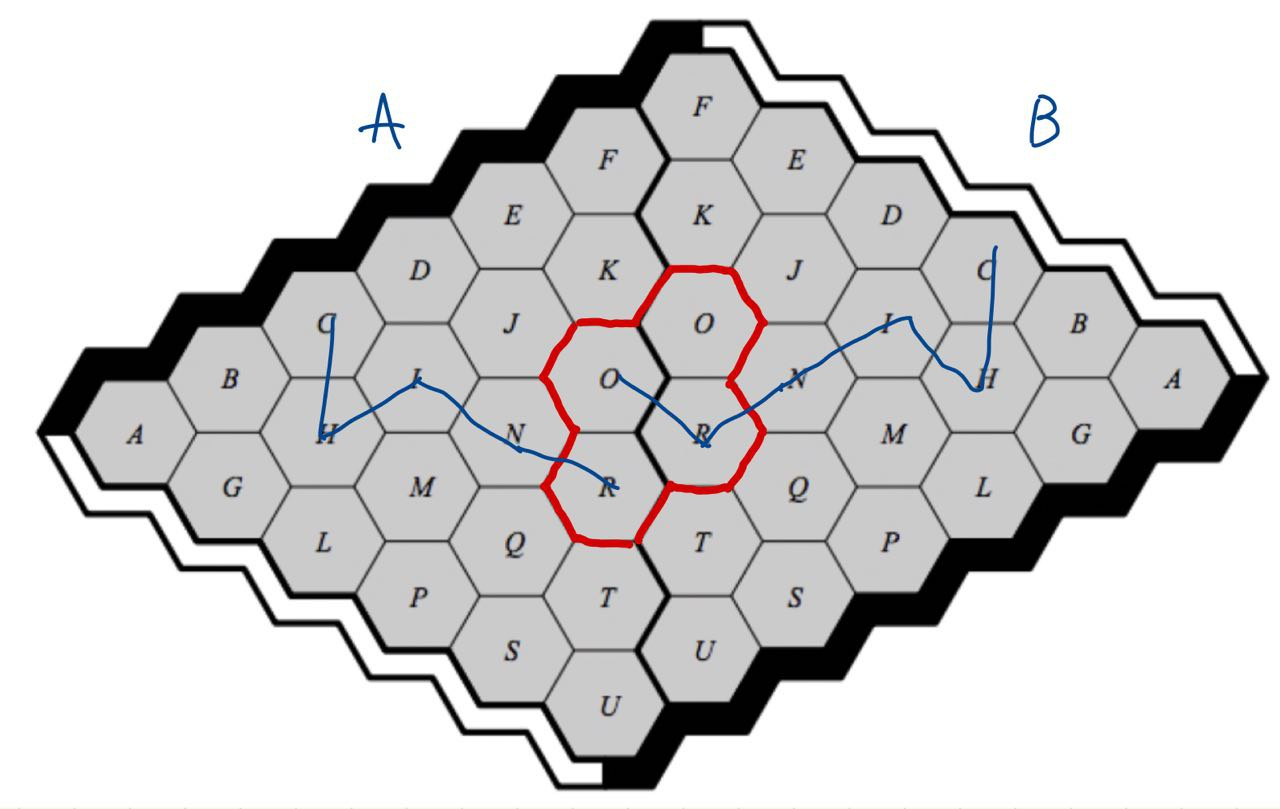
\includegraphics[width=0.7\linewidth]{hex}
	\caption{This figure shows that A (the longer side) always win the hex game no matter it is black or white using the mirror strategy.}
	\label{fig:hex}
\end{figure}

\begin{code}
\captionof{listing}{A Python code block}
\label{code: extract}
\begin{minted}
from sqlite3 import Timestamp
import cv2
import time

cap = cv2.VideoCapture("DSCF9363.mp4")

tum_file = open("dorm_tum.txt", "w")
frame_rate = 59.94
timestamp = time.time()
i = 0
while cap.isOpened():
    ret, frame = cap.read()
    if not ret:
        break
    if i % 5 == 0:
        tum_file.write(f"{timestamp} dorm_video/{i}.png\n")
        cv2.imwrite(f"dorm_video/{i}.png", frame)
    i += 1
    timestamp += 1.0 / frame_rate

tum_file.close()
\end{minted}
\end{code}

\end{document}